%------------------------------------------------------------%

\chapter{Desenvolvimento}
\label{cap:trabalhos:desenvolvimento}

Este capítulo apresenta o desenvolvimento do sistema robótico proposto, abrangendo tanto os aspectos de hardware quanto os de software. Inicialmente, são descritas as características físicas e funcionais da plataforma robótica desenvolvida, incluindo alguns detalhes sobre a estrutura mecânica, os sensores embarcados e os sistemas de controle e comunicação utilizados. Também são apresentados os dois outros protótipos empregados durante as fases de simulação, com destaque para suas diferenças estruturais e contribuições ao processo de validação. Em seguida, é detalhada a configuração dos sensores no ambiente ROS, abordando os drivers utilizados, os parâmetros operacionais ajustados e as estratégias adotadas para formatar os dados obtidos em diferentes plataformas. Posteriormente, são explorados os aspectos de software, incluindo o controle do robô via ROS, o processamento e organização dos dados adquiridos e a implementação dos modelos de aprendizado de máquina. Todo o pipeline, desde a aquisição até a inferência em tempo real, foi projetado para ser modular, adaptável e compatível tanto com simulações quanto com a operação embarcada em plataformas reais.

\section{Hardware}

Esta seção descreve os aspectos físicos e estruturais do sistema robótico desenvolvido, incluindo detalhes da construção mecânica do robô utilizado para a coleta de dados reais, os protótipos testados em simulação, e a configuração do suporte dos sensores multimodais. São apresentados também os sensores utilizados e suas principais especificações técnicas.

\subsection{Estrutura Mecânica dos Robôs}

O robô utilizado na coleta de dados em ambiente real foi construído com estrutura impressa em 3D, baseada no mesmo modelo utilizado nas simulações desenvolvidas no CoppeliaSim. Seu deslocamento ocorre sobre um cabo rígido, representando uma linha de transmissão, e utiliza dois motores de passo: um responsável pelo deslocamento linear ao longo do cabo e outro para acionar o mecanismo de travamento/destravamento. Este mecanismo garante que o robô permaneça fixo ao cabo, impedindo quedas ou movimentos involuntários durante a coleta de dados.

Este modelo apresenta uma estrutura simplificada e não conta com sistemas embarcados para a superação de obstáculos. A escolha por este robô para a coleta de dados se deu por sua maior confiabilidade estrutural, sendo o mais estável dentre os disponíveis no laboratório. A proposta para uma versão final inclui a adição de um segundo conjunto de garra e um corpo robusto capaz de sustentar o robô com apenas uma garra acoplada. Em presença de obstáculos, a ideia é que o robô desacople uma das garras, rotacione-a para ultrapassar o obstáculo, recoloque-a no cabo após o objeto e, em seguida, repita o processo com a outra garra, garantindo a continuidade do deslocamento.

Além do protótipo utilizado na coleta real, dois outros robôs com mecanismos funcionais de superação de obstáculos foram projetados e simulados. O primeiro deles é composto por um corpo central com duas rodas laterais e uma garra central. Quando detecta um obstáculo, a garra se prende ao cabo, a roda dianteira se desacopla, desce, e o corpo do robô se estende para reposicionar a roda à frente do obstáculo. Após reposicionada, a roda retorna à altura do cabo, se fecha e o robô solta a garra, retrai o corpo e avança, repetindo o processo com a outra roda para completar a travessia do obstáculo.

O segundo robô possui três braços articulados, cada um equipado com rodas e um “cotovelo” acionável. Ao detectar um obstáculo, o primeiro braço eleva seu cotovelo e ultrapassa o obstáculo. Em seguida, os outros dois braços repetem o movimento sequencialmente, permitindo que o robô supere a barreira mantendo estabilidade e tração no cabo. Apesar da complexidade desses mecanismos, a instabilidade estrutural observada nos protótipos reais inviabilizou sua utilização na coleta física de dados, sendo restritos às simulações computacionais.

\subsection{Sensor Multimodal}

Para este projeto, foi construído um suporte físico com o objetivo de manter fixas a orientação e a posição dos sensores utilizados. O suporte foi projetado com o menor tamanho possível, desde que não comprometesse a estabilidade dos sensores. A escolha das posições relativas entre os sensores foi determinada com base em seus papéis específicos dentro do sistema robótico e nas exigências geométricas para uma coleta eficiente dos dados.

O sensor LiDAR tem como principal função levantar informações de profundidade ao redor da linha, sendo, portanto, essencial que ele possua uma visão desobstruída do ambiente. Para maximizar a utilidade das suas leituras, o plano de varredura do sensor deve estar livre de rotações em relação ao eixo da linha. Além disso, o ângulo do plano de leitura não pode ser muito próximo ao da própria linha, pois isso limitaria a abrangência das medições. Idealmente, o plano do LiDAR estaria orientado a $90^\circ$ em relação ao eixo do cabo, oferecendo uma visão lateral completa do entorno. No entanto, para que o robô seja capaz de detectar e classificar objetos à sua frente antes de se aproximar demasiadamente, é necessário inclinar o sensor em relação ao eixo do cabo. O melhor caso, nesse sentido, seria o sensor operando a $0^\circ$ em relação ao eixo do cabo, mirando diretamente à frente. (Figura para demonstrar?)

A câmera de profundidade também tem papel relevante na análise da linha e dos objetos presentes nela, sendo usada principalmente para detecção de possíveis danos físicos. Para evitar distorções e maximizar a qualidade das imagens, a câmera deve ser posicionada acima do cabo, com seu plano óptico perpendicular ao eixo da linha e voltado para frente.

Considerando os requisitos específicos de cada sensor, o suporte multimodal foi projetado para equilibrar as limitações de ambos. O ângulo de fixação do LiDAR foi definido como $45^\circ$ em relação ao eixo do cabo. Essa inclinação permite a coleta tanto de dados laterais quanto frontais, desde que o sensor esteja a uma distância horizontal adequada em relação ao cabo. A câmera foi posicionada na parte superior do robô, acima do cabo, a uma distância de $5\,\text{cm}$ a partir do centro do mesmo. (Figura com as medidas)

Foi estabelecido que a classificação dos objetos deve ser feita a partir da leitura combinada de ambos os sensores. Como a câmera de profundidade possui maior alcance visual em relação ao LiDAR (devido à sua posição elevada), definiu-se uma distância mínima de $40\,\text{cm}$ para a detecção e classificação de objetos. Ou seja, qualquer objeto a $40\,\text{cm}$ ou menos da frente do robô deve ser processado pelo sistema multimodal.

Para garantir essa faixa de detecção, o suporte foi projetado com $50\,\text{cm}$ de comprimento horizontal, mantendo o LiDAR a $45\,\text{cm}$ abaixo do cabo (a partir do seu centro) e a câmera a $5\,\text{cm}$ acima. Essa configuração assegura que o LiDAR possa detectar objetos a mais de $45\,\text{cm}$ de distância, caso estejam abaixo do cabo, e objetos a pelo menos $40\,\text{cm}$ se estiverem posicionados ligeiramente acima da linha. Dessa forma, o arranjo garante a eficácia do sistema de classificação sem comprometer a integridade ou a estabilidade do robô durante o deslocamento.

\subsection{Sensores Utilizados}

Para a realização deste projeto, foram selecionados dois sensores principais capazes de fornecer informações de profundidade complementares: a câmera Intel RealSense D415 e o LiDAR RPLIDAR A1M8. Ambos os sensores foram integrados ao sistema embarcado do robô para permitir a coleta de dados tridimensionais, usados para a tarefa de classificação de objetos sobre as linhas de transmissão. A escolha por sensores de profundidade com diferentes princípios de funcionamento — estereoscopia ativa e triangulação a laser — visa garantir robustez ao sistema em diferentes condições de iluminação, ângulos de incidência e posicionamentos relativos dos objetos. A seguir, são descritas as principais características técnicas de cada sensor.

\subsubsection{Intel RealSense D415}

A câmera de profundidade Intel RealSense D415 utiliza um sistema estereoscópico ativo para gerar mapas de profundidade com alta precisão. A tecnologia baseia-se na captura simultânea de imagens por duas câmeras infravermelhas, associadas a um projetor de padrões que melhora a detecção em superfícies com baixo contraste visual. Essa configuração permite estimar a profundidade por meio da disparidade entre os pares de imagens. O sensor é amplamente empregado em aplicações de robótica, visão computacional e automação, dada sua confiabilidade e facilidade de integração com plataformas embarcadas.

% \begin{figure}[!h]
%     \centering
%     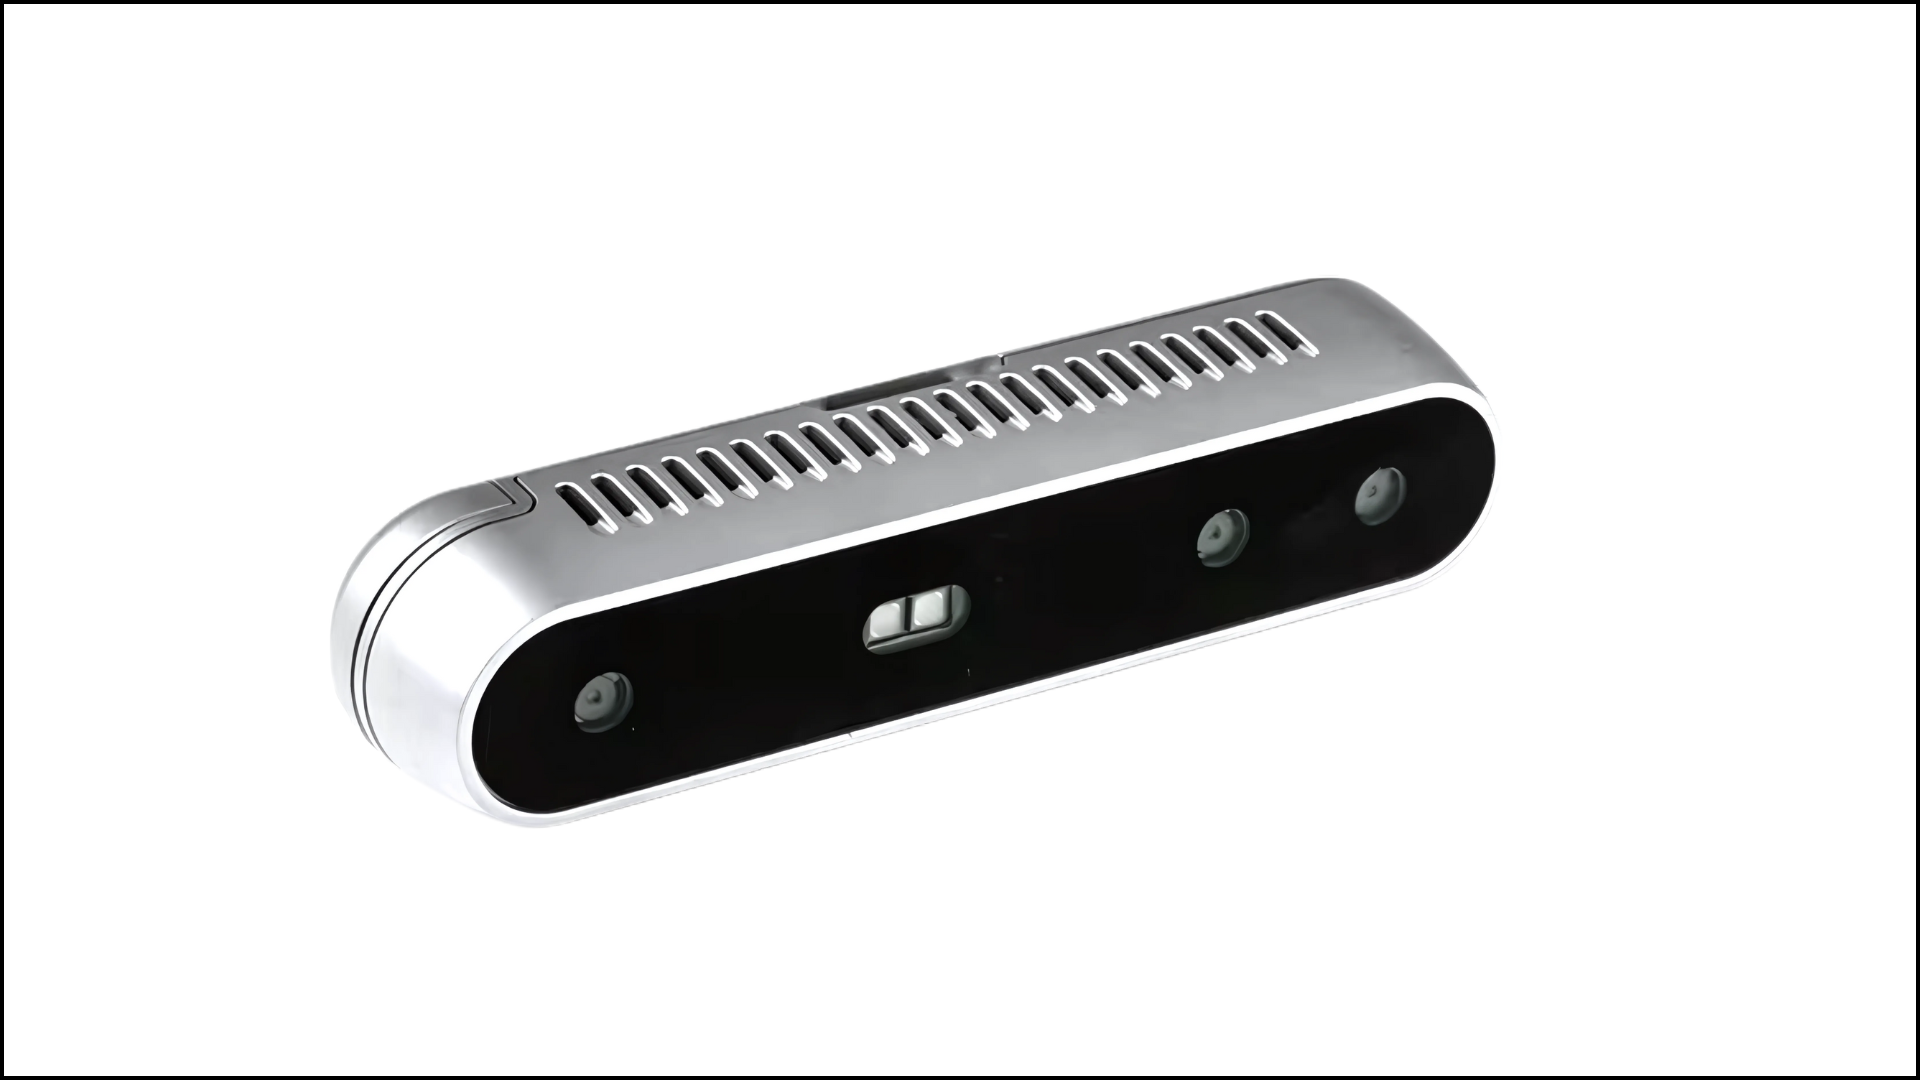
\includegraphics[width=0.4\columnwidth]{RealSense.jpg}
%     \caption{Intel RealSense D415}
%     \label{fig:realsense-D415}
% \end{figure}

As principais especificações técnicas da RealSense D415 incluem:

\begin{itemize}
    \item \textbf{Tecnologia de profundidade}: Estereoscopia ativa com projetor infravermelho
    \item \textbf{Distância mínima de operação}: Aproximadamente $0{,}45\,\text{m}$ para resolução máxima
    \item \textbf{Precisão de profundidade}: Erro inferior a $2\%$ a $2\,\text{m}$
    \item \textbf{Campo de visão (FOV)}: $65^\circ \times 40^\circ$
    \item \textbf{Resolução de saída}: Até $1280 \times 720$ pixels
    \item \textbf{Taxa de quadros (depth)}: Até $90\,\text{fps}$
\end{itemize}

\subsubsection{RPLIDAR A1M8}

O sensor RPLIDAR A1M8, desenvolvido pela Slamtec, é um sensor LiDAR de baixo custo que opera por meio da técnica de triangulação a laser infravermelho. Sua principal funcionalidade está na realização de escaneamentos 2D em $360^\circ$, sendo capaz de gerar nuvens de pontos com alta densidade. Devido à sua leveza, baixo consumo energético e boa precisão, o sensor é amplamente empregado em sistemas de navegação autônoma e mapeamento em tempo real (SLAM). Um motor rotativo interno aciona o movimento contínuo do feixe de laser, permitindo medições em tempo real com ampla cobertura angular.

As principais especificações técnicas do RPLIDAR A1M8 são:

\begin{itemize}
    \item \textbf{Tecnologia de medição}: Triangulação com laser infravermelho
    \item \textbf{Alcance de detecção}: $0{,}15\,\text{m}$ a $12\,\text{m}$
    \item \textbf{Campo de visão (FOV)}: $360^\circ$ contínuo
    \item \textbf{Frequência de varredura}: $10\,\text{Hz}$
    \item \textbf{Resolução angular}: $\leq 1^\circ$
    \item \textbf{Frequência de amostragem}: $\geq 8000$ pontos por segundo
    \item \textbf{Precisão de distância}: Erro inferior a $1\%$ da distância medida
    \item \textbf{Interface de comunicação}: UART (TTL $3{,}3\,\text{V}$)
\end{itemize}

\section{Firmware e Software}

O funcionamento do sistema proposto depende da integração eficiente entre o hardware embarcado, os sensores e os algoritmos de controle e aquisição de dados. Para isso, foi desenvolvido um conjunto de códigos em Python e C++ utilizando o framework ROS, que facilita a comunicação entre os diversos componentes do sistema. O firmware, executado na placa Arduino, é responsável apenas pela interface direta com os drivers dos motores, enquanto o software, executado na Raspberry Pi, gerencia os sensores, o controle dos atuadores e a coleta dos dados. As seções a seguir descrevem detalhadamente a configuração dos sensores, a estrutura de controle dos robôs, tanto em ambiente simulado quanto real, e o script de coleta e armazenamento dos dados utilizados no treinamento dos modelos de classificação.

\subsection{Controle do Robô via ROS}

O controle dos motores foi realizado por meio de um microcontrolador Arduino, que funcionou como interface entre o sistema ROS e os drivers dos motores. Para essa comunicação, foi criado um tópico específico no ROS, no qual as mensagens eram do tipo \texttt{std\_msgs/Int64MultiArray}. Cada posição do vetor representava um motor, e seu valor indicava, conforme a topologia do robô, a velocidade ou o número de passos a ser executado. O Arduino recebia os comandos por meio da porta serial e os repassava aos motores, sendo responsável apenas pela comunicação com os drivers. Nenhuma lógica de controle era executada no próprio Arduino, ficando essa tarefa completamente a cargo dos nós do ROS.

No robô utilizado para aquisição dos dados, existiam dois elementos principais de controle: a trava de segurança e o motor responsável pelo deslocamento linear ao longo da linha de transmissão. A trava recebia, por meio do vetor de controle, o número de passos necessários para travar e destravar o robô no cabo condutor. O motor de movimentação, por sua vez, recebia a velocidade desejada. O código de controle desenvolvido no ROS impedia que o robô iniciasse o movimento sem que a trava estivesse acionada, garantindo a segurança da estrutura e prevenindo quedas.

Para os robôs utilizados nas simulações, foram adotados os mesmos códigos utilizados no robô físico, com adaptações no tamanho do vetor de controle para refletir o número de atuadores presentes em cada topologia. O robô simulado utilizado na aquisição de dados operava de forma idêntica ao robô real, enquanto outras topologias simuladas apresentavam variações no número de motores ou atuadores, mantendo, contudo, o mesmo princípio de controle por meio de tópicos ROS e vetores de comandos.

\subsection{Configuração dos Sensores}

Na simulação, foram utilizados modelos de sensores que reproduzem as mesmas características dos sensores reais adotados na implementação prática. As configurações foram realizadas por meio das bibliotecas \texttt{rplidar\_ros} e \texttt{realsense2\_camera}, disponíveis no ecossistema do ROS. Para o LiDAR, não foram necessárias modificações adicionais, pois a configuração padrão já atendia aos requisitos do projeto. No caso da câmera RealSense D415, foi ajustada para operar a uma taxa de 10~Hz e com resolução de 1280$\times$720 pixels, de modo a sincronizar sua aquisição com o LiDAR. Essa configuração resultou em uma distância mínima de leitura de aproximadamente 4,5 centímetros.

Uma vez configurados e iniciados os respectivos nós dos sensores, os dados passaram a ser publicados nos tópicos definidos pelas bibliotecas. O sensor LiDAR publica mensagens do tipo \texttt{sensor\_msgs/LaserScan}, que consistem em uma estrutura padronizada para representar leituras de distância obtidas por varredura a laser. Essa mensagem contém informações como o ângulo inicial (\texttt{angle\_min}) e final (\texttt{angle\_max}) da varredura, o incremento angular entre medições (\texttt{angle\_increment}), a distância mínima (\texttt{range\_min}) e máxima (\texttt{range\_max}) detectáveis, e o vetor \texttt{ranges}, que armazena as distâncias medidas, em metros, para cada ângulo. Opcionalmente, o campo \texttt{intensities} pode conter dados referentes à intensidade do sinal refletido, útil para análise de propriedades ópticas dos objetos. O campo \texttt{header}, presente em todas as mensagens ROS, fornece informações de carimbo de tempo e identificação do sistema de coordenadas (\texttt{frame\_id}) associado à leitura.

Para os sensores de visão, como a câmera de profundidade RealSense, os dados são publicados em tópicos do tipo \texttt{sensor\_msgs/Image}. Essa mensagem carrega as imagens ou quadros de vídeo capturados e contém metadados como a resolução da imagem (\texttt{width} e \texttt{height}), o número de bytes por linha (\texttt{step}) e os dados brutos da imagem no campo \texttt{data}. A codificação dos pixels é especificada no campo \texttt{encoding}, com formatos comuns como \texttt{"rgb8"}, \texttt{"bgr8"}, \texttt{"mono8"} ou \texttt{"yuv422"}. O campo \texttt{is\_bigendian} informa a ordem dos bytes utilizada. Neste projeto, foram utilizadas imagens em escala de cinza (\textit{grayscale}), com codificação de 8 bits por pixel para os dados simulados e de 16 bits por pixel para os dados adquiridos em ambiente real.

\subsection{Script de Coleta}

O script de coleta de dados foi desenvolvido em \textit{Python}, com o objetivo de registrar as informações publicadas nos tópicos dos sensores utilizados. Para a câmera de profundidade, o script armazenava diretamente as imagens geradas, enquanto, para o LiDAR real, era aplicado um pré-processamento com a finalidade de restringir o campo de leitura do sensor.

Esse pré-processamento consistia em limitar o ângulo de leitura para um setor de 10 graus, centrado à frente do sensor, de modo que apenas as amostras dentro desse intervalo fossem consideradas. Como resultado, cada varredura do LiDAR fornecia 63 leituras, correspondentes a esse setor angular reduzido.

Após iniciado, o script realizava a inscrição nos tópicos dos sensores e armazenava os dados recebidos. Como ambos os sensores estavam configurados para operar a uma frequência de 10 Hz, os dados capturados já estavam naturalmente sincronizados no tempo, dispensando a necessidade de sincronização adicional. O script permanecia em execução até atingir o número desejado de amostras, que, neste caso, foi de 160 registros por objeto observado.

\section{Coleta dos Dados}

Para a coleta dos dados, os objetos foram posicionados um a um em frente aos sensores, de modo que ficassem visíveis tanto para o LiDAR quanto para a câmera de profundidade. Em seguida, o robô era aproximado gradualmente até que o sensor LiDAR passasse a registrar leituras referentes ao objeto. Nesse momento, o script de coleta era iniciado, e o robô começava a se deslocar lentamente em direção ao objeto, conforme ilustrado na Figura%~\ref{fig:coleta_dados}.

% \begin{figure}[!h]
%     \centering
%     \includegraphics[width=0.75\textwidth]{figs/coleta_dados.png}
%     \caption{Representação do processo de coleta de dados com o objeto posicionado à frente dos sensores.}
%     \label{fig:coleta_dados}
% \end{figure}

A velocidade de deslocamento era ajustada individualmente para cada objeto, com o intuito de capturar a maior variedade possível de distâncias ao longo da aproximação. A coleta era interrompida somente quando o robô alcançava a última posição em que ambos os sensores ainda conseguiam registrar o objeto de forma eficaz. Considerando que os sensores operavam a uma taxa de 10 Hz, cada sessão de coleta durava 16 segundos, o que resultava em 160 amostras por objeto.

Ao todo, foram coletadas 1.280 imagens de profundidade e 80.640 leituras de distância do LiDAR provenientes do robô principal (dados reais e simulados). Além disso, foram obtidas 640 imagens de profundidade e 40.320 leituras de distância de dados simulados de cada um dos dois robôs utilizados para validar a abordagem multimodal. Os dados foram organizados em quatro classes: amortecedor, isolador, sinalizador e nada.

A partir dessas coletas, foram criados cinco \textit{datasets} distintos para cada origem de dado, totalizando 4 conjuntos por tipo de topologia (principal [simulado e real], secundárias [simulado]). Esses conjuntos compreendem: (i) imagens brutas da câmera de profundidade; (ii) dados brutos do LiDAR; (iii) \textit{features} extraídas das imagens de profundidade; (iv) \textit{features} extraídas dos dados do LiDAR; e (v) uma junção das \textit{features} das duas modalidades. Essa organização foi essencial para a análise comparativa entre sensores e para o desenvolvimento de modelos capazes de explorar diferentes níveis de abstração e fusão de dados.

\section{Processamento de Dados}

Nesta seção são apresentadas as técnicas empregadas no processamento dos dados coletados pelos sensores, com foco na extração de \textit{features} relevantes para a classificação dos objetos. Também são descritos os métodos utilizados para a organização e construção dos conjuntos de dados (datasets) utilizados no treinamento dos modelos de aprendizado de máquina.

Para ambos os sensores — LiDAR e câmera de profundidade — foram aplicadas etapas de pré-processamento com o objetivo de reduzir ruídos e tornar os dados mais consistentes. Inicialmente, valores discrepantes (outliers) foram removidos, e todos os dados brutos foram truncados para conter 150 elementos, de forma a padronizar as entradas para os classificadores. Os trechos a seguir detalham os procedimentos adotados para cada sensor individualmente, abordando tanto a estrutura dos dados coletados quanto o processo de extração de características específicas (\textit{features}) que representam propriedades dos objetos observados.

\subsection{Dados do LiDAR}

Os dados coletados pelo sensor LiDAR foram armazenados em arquivos no formato de tabela, onde cada linha representa uma varredura completa (ou \textit{scan}) do sensor, e cada coluna corresponde a um ângulo específico da leitura. O campo de visão considerado para o processamento foi de $10^\circ$, centrado na frente do sensor, isto é, de $-5^\circ$ a $+5^\circ$, totalizando 63 amostras por varredura. As distâncias registradas variam entre 0 e 12 metros.

Para compor os vetores de características (\textit{features}) utilizados nos modelos de classificação, foram extraídas duas informações principais de cada varredura do sensor:

\begin{itemize}
    \item \textbf{Número de leituras consecutivas representando o objeto}: Essa \textit{feature} corresponde à quantidade de amostras dentro de uma varredura que indicam a presença de um objeto. A ideia é que, quando o sensor não detecta nenhum objeto, ele retorna valores equivalentes ao "fundo de escala", ou seja, a distância máxima possível (12 metros). Isso é válido nos dados simulados, onde o ambiente é aberto, mas não se aplica diretamente ao laboratório real, onde o sensor pode registrar leituras de até 2 metros devido à proximidade de paredes e objetos. Além disso, quando o sensor real não consegue realizar a leitura, ele também retorna valores máximos. Para contornar esse problema, o algoritmo começa analisando a primeira leitura da varredura e a compara com a seguinte. Se forem iguais, assume-se que o sensor ainda não detectou um objeto. A detecção do início do objeto só é confirmada se as duas próximas leituras forem diferentes. A partir daí, o algoritmo continua até identificar o retorno ao valor inicial (indicando o fim do objeto), contando o número de amostras distintas do fundo de escala. Esse valor é proporcional ao diâmetro aparente do objeto: quanto maior o objeto, maior o número de leituras consecutivas representando sua presença.
    
    \item \textbf{Distância média do objeto}: Após identificado o intervalo das leituras correspondentes ao objeto, é calculada a média desses valores. Essa média representa a distância média entre o objeto e o sensor LiDAR durante aquela varredura. Essa \textit{feature} é importante para distinguir objetos que, mesmo com tamanhos semelhantes, são posicionados a distâncias diferentes.
\end{itemize}

\subsection{Dados da RealSense}

Para o processamento das imagens de profundidade obtidas pela câmera Intel RealSense D415, foram adotadas técnicas leves de extração de \textit{features}, visando a viabilidade de uso em sistemas embarcados com recursos computacionais limitados. Dessa forma, evitou-se o uso de redes convolucionais complexas para as etapas iniciais de processamento.

Inicialmente, todas as imagens foram redimensionadas para $460 \times 460$ pixels. Como a posição relativa do robô em relação aos objetos de interesse era fixa, essa janela foi suficiente para capturar os objetos com boa visibilidade e, ao mesmo tempo, reduzir o custo de processamento.

\subsubsection{Limite de profundidade}

A primeira etapa do processamento consistiu na aplicação de um limite de profundidade às imagens. Essa técnica atua como uma forma de segmentação grosseira, onde apenas objetos posicionados até uma certa distância da câmera são considerados relevantes. O limite escolhido foi de 1 metro.

No caso das imagens simuladas (com 8 bits por pixel, variando de 0 a 255 para representar 0 a 12 metros), esse corte foi feito fixando o valor de 22 como o limite superior. Assim, pixels com valores acima de 22 foram convertidos para 0, descartando regiões além de 1 metro. Para as imagens reais (com 16 bits por pixel, onde cada unidade representa 1 mm), o valor limite foi definido como 1000, seguindo a mesma lógica.

Após essa filtragem, restaram apenas os pixels associados aos objetos de interesse, facilitando a extração de características. As primeiras \textit{features} extraídas foram a média e a variância dos valores dos pixels remanescentes, refletindo respectivamente a distância média dos objetos e a sua dispersão na imagem.

\subsubsection{Preparação das imagens para a rede SqueezeNet}

As imagens simuladas, devido à sua codificação simples, foram diretamente utilizadas para o treinamento da SqueezeNet. No entanto, as imagens reais apresentavam baixa luminosidade aparente devido à sua codificação em profundidade de 16 bits, o que dificultava sua interpretação visual e o uso direto em redes neurais.

Para resolver esse problema, foi aplicada a técnica de \textbf{equalização de histograma}, que visa melhorar o contraste da imagem redistribuindo os valores de intensidade. Essa técnica reatribui os níveis de cinza de forma que o histograma da imagem se aproxime de uma distribuição uniforme. Com isso, detalhes que antes estavam comprimidos em faixas de intensidade estreitas passam a ser mais destacados, tornando a imagem mais nítida para o aprendizado da rede.

\subsubsection{Contorno dos objetos}

Outra \textit{feature} extraída das imagens foi a quantidade de pixels localizados nas bordas dos objetos. Para isso, foi aplicado o \textbf{filtro Laplaciano}, um operador de detecção de bordas baseado na segunda derivada da imagem, que enfatiza regiões onde ocorrem mudanças abruptas de intensidade — ou seja, as bordas dos objetos. Foi aplicado um filtro com um \textbf{kernel} pequeno (3x3), que define a área da imagem analisada por vez na aplicação do operador (neste caso, o filtro Laplaciano). O \textit{kernel} funciona como uma matriz que percorre a imagem, realizando operações locais — quanto menor o kernel, mais local é a detecção de variações. Como os valores dos pixels não foram multiplicados por um fator de ganho, apenas as bordas mais marcantes dos objetos foram evidenciadas, já que a imagem eram valores de profundidade as variações entre pixels era pequena se analisada em locais referentes ao mesmo objeto.

Em seguida, a imagem foi \textbf{binarizada}, convertendo todos os valores com variação maior que 20 centímetros para 1 e o resto para 0, o que resultou em uma imagem que destaca apenas os contornos principais dos objetos. Em seguida, contou-se o número total de pixels com valor 1, o que fornece uma estimativa do perímetro dos objetos.

\subsubsection{Operações morfológicas}

A última \textit{feature} extraída baseou-se em operações morfológicas aplicadas sobre a imagem com o limite de profundidade. Primeiramente, a imagem foi binarizada, com todos os pixels diferentes de zero convertidos em 1. Em seguida, foram aplicadas duas operações:

\begin{itemize}
    \item \textbf{Fechamento}: operação composta por uma dilatação seguida de erosão. Serve para preencher pequenos buracos e eliminar pequenos vazios internos nos objetos, unificando contornos desconexos.
    \item \textbf{Abertura}: operação composta por uma erosão seguida de dilatação. Tem como função remover pequenos ruídos e detalhes irrelevantes, suavizando os contornos dos objetos.
\end{itemize}

Essas operações foram aplicadas duas vezes: uma com um \textbf{kernel grande} ($15 \times 15$), o que resulta em uma suavização mais agressiva, unificando áreas extensas e eliminando ruídos significativos; e outra com um \textbf{kernel pequeno} ($2 \times 2$), que atua de forma mais sutil, preservando detalhes finos.

Ao final dessas operações, a imagem resultante continha apenas a silhueta binária dos objetos principais. A contagem do número de pixels com valor 1 nessa imagem foi utilizada como a última \textit{feature}, representando a área total ocupada pelo objeto visível ao sensor.

% \begin{figure}[!h]
%     \centering
%     \includegraphics[width=0.8\textwidth]{figuras/exemplo_features_realsense.png}
%     \caption{Exemplo de imagem de profundidade e etapas de extração de \textit{features}.}
%     \label{fig:features_realsense}
% \end{figure}

\section{Treinamento e Validação}

Nesta seção são apresentadas as configurações utilizadas para o treinamento dos modelos de aprendizado de máquina, bem como os procedimentos adotados para validação dos mesmos. Inicialmente, são detalados os parâmetros e arquiteturas de cada um dos classificadores utilizados neste trabalho, com justificativas para as escolhas feitas em cada caso. Em seguida, são descritos os dois métodos de validação empregados: o primeiro, com validação cruzada, busca avaliar o desempenho dos modelos com os próprios dados coletados; o segundo testa a capacidade dos modelos em generalizar para novas topologias de sensores, avaliando sua portabilidade em cenários distintos daquele utilizado no treinamento.

\subsection{Configuração dos Modelos}

Nesta subseção são descritas as configurações específicas adotadas para cada um dos modelos de classificação utilizados no experimento. Os modelos foram selecionados por sua ampla utilização em problemas de classificação supervisionada. Para cada modelo, são detalhados os hiperparâmetros ajustados, as estratégias de pré-processamento aplicadas e, quando relevante, as características particulares da implementação. As escolhas foram feitas com o objetivo de equilibrar desempenho, simplicidade e viabilidade de implementação em sistemas embarcados.

\subsubsection{Árvore de Decisão}

O classificador de Árvore de Decisão foi utilizado com as configurações padrão oferecidas pela biblioteca \textit{scikit-learn}, exceto pelo parâmetro \texttt{random\_state}, definido como 42 para garantir a reprodutibilidade dos resultados. A profundidade máxima da árvore foi mantida ilimitada (\texttt{max\_depth=None}), permitindo a expansão dos nós até que todas as folhas fossem puras. O número mínimo de amostras necessário para realizar uma divisão foi fixado em 2 (\texttt{min\_samples\_split=2}), enquanto o número mínimo de amostras exigido para formar uma folha foi mantido em 1 (\texttt{min\_samples\_leaf=1}). A quantidade máxima de características consideradas por divisão foi deixada como \texttt{None}, indicando que todas estavam disponíveis para análise em cada nó.

Esses parâmetros favorecem o sobreajuste aos dados de treinamento, mas esse comportamento não é problemático no contexto deste trabalho, visto que os dados seguem um padrão bem definido. O critério de divisão adotado foi o índice Gini (\texttt{criterion='gini'}), amplamente utilizado por sua simplicidade e eficiência. A estratégia de seleção das divisões foi a \texttt{'best'}, escolhendo a característica e o valor de corte que maximizam a redução da impureza em cada nó.

\subsubsection{k-Vizinhos mais proximos}

Para o classificador kNN, foi adotado o valor de $k=3$, ou seja, a classe atribuída a uma nova amostra é determinada com base nas três amostras mais próximas no conjunto de treinamento. A métrica utilizada para o cálculo das distâncias foi a distância Euclidiana, devido à sua simplicidade e adequação a espaços vetoriais contínuos. Todos os vizinhos tiveram o mesmo peso na votação (\texttt{weights='uniform'}), o que significa que cada um dos $k$ vizinhos contribui igualmente para a decisão da classe final.

\subsubsection{Naive Bayes}

Foi utilizado o classificador \texttt{GaussianNB}, que assume que as características seguem uma distribuição normal (gaussiana). As probabilidades a priori das classes foram consideradas iguais, com o parâmetro \texttt{priors} definido como $[0{,}25,\ 0{,}25,\ 0{,}25,\ 0{,}25]$. O parâmetro \texttt{var\_smoothing}, responsável por suavizar a variância e evitar instabilidades numéricas, foi mantido em seu valor padrão de $1 \times 10^{-9}$. 

\subsubsection{Random Forest}

O classificador de Floresta Aleatória foi configurado com 100 estimadores (\texttt{n\_estimators=100}), ou seja, o modelo é composto por 100 árvores de decisão independentes. O parâmetro \texttt{random\_state} foi fixado em 42 para garantir reprodutibilidade. Os demais hiperparâmetros foram mantidos nos valores padrão da biblioteca, incluindo profundidade ilimitada (\texttt{max\_depth=None}), divisão mínima de duas amostras (\texttt{min\_samples\_split=2}), critério Gini (\texttt{criterion='gini'}) e amostragem com reposição (\texttt{bootstrap=True}).

Além disso, foi incluído um estágio de normalização no pipeline utilizando o \texttt{StandardScaler}, que transforma as características para média zero e desvio padrão unitário, contribuindo para o equilíbrio das variáveis no treinamento.

\subsubsection{Rede Neural}

A arquitetura de rede neural densa utilizada foi composta por três camadas totalmente conectadas, intercaladas com funções de ativação ReLU. A primeira camada oculta contém 128 neurônios, a segunda 64, e a camada de saída possui 4 neurônios, correspondentes às quatro classes do problema. Foi utilizada a função de perda \texttt{CrossEntropyLoss}, adequada para tarefas de classificação multiclasse, e o otimizador \texttt{Adam} com taxa de aprendizado de 0{,}001.

O treinamento foi realizado por até 200 épocas, com tamanho de lote (\texttt{batch\_size}) de 32 amostras. Implementou-se ainda uma estratégia de parada antecipada, que interrompe o treinamento caso a perda média da época fosse inferior a 0{,}001.

\subsubsection{SqueezeNet}

A arquitetura SqueezeNet foi adaptada para este trabalho pela modificação de sua camada final, ajustando o número de saídas para 4 (\texttt{num\_classes=4}). O treinamento foi realizado com a função de perda \texttt{CrossEntropyLoss} e o otimizador \texttt{Adam}, com taxa de aprendizado de 0{,}001. O processo de treinamento foi conduzido por até 100 épocas, com lotes de 16 amostras (\texttt{batch\_size=16}).

Foi empregada uma estratégia de parada antecipada caso a perda média por época atingisse valor inferior a 0{,}001. Todas as imagens utilizadas foram redimensionadas para $224 \times 224$ pixels e normalizadas com média e desvio padrão iguais a 0{,}5, de acordo com as recomendações usuais para esse tipo de arquitetura.

\subsection{Validação}

Foram realizados dois testes distintos para validação dos modelos de classificação. O primeiro teve como objetivo verificar se os dados coletados eram suficientemente representativos para permitir a distinção entre as classes. O segundo visou avaliar a portabilidade dos modelos treinados, bem como a capacidade do sensor multimodal de generalizar os resultados para diferentes topologias robóticas.

No primeiro teste, foi aplicada a técnica de validação cruzada com 5 dobras (\textit{5-fold cross-validation}). O conjunto de dados foi dividido em cinco partes, mantendo a distribuição de classes equilibrada — cada uma das quatro classes apresentou 30 amostras em cada divisão, totalizando 120 amostras por dobra. Em cada iteração da validação cruzada, quatro partes foram utilizadas para o treinamento e a parte restante, que não participou do treinamento, foi usada para validação. Esse processo foi repetido cinco vezes, garantindo que todas as subdivisões fossem utilizadas como conjunto de validação uma vez.

Durante cada validação, foram registradas as seguintes métricas:
\begin{itemize}
    \item \textbf{Acurácia da dobra}: proporção de classificações corretas sobre o total de amostras;
    \item \textbf{Perda (Loss)} e \textbf{época final}: quando aplicável, indicam a performance do modelo ao final do treinamento;
    \item \textbf{Tempo de validação}: tempo necessário para que o modelo, já treinado, classificasse as 120 amostras da dobra de validação;
    \item \textbf{Matriz de confusão}: registrou-se, para cada modelo treinado, a matriz de confusão resultante, com o intuito de identificar padrões de erro na classificação.
\end{itemize}

A matriz de confusão apresenta, para cada classe, a quantidade de amostras corretamente classificadas (na diagonal principal) e os erros de classificação (nas demais posições), permitindo uma análise detalhada do desempenho do modelo em cada classe individualmente.

O segundo teste de validação teve como foco a verificação da portabilidade dos modelos e da robustez do sensor multimodal frente a diferentes topologias robóticas. Os modelos foram treinados exclusivamente com os dados obtidos na simulação da primeira topologia. Em seguida, os dados das outras duas topologias foram utilizados como conjuntos de validação independentes.

As métricas registradas foram as mesmas do primeiro teste — acurácia, perda final, época final (quando aplicável) e tempo de validação. A diferença principal foi o número de amostras envolvidas: cada topologia forneceu 600 dados para validação, tornando essa avaliação mais robusta em termos estatísticos.


%-----------------------------------------------------------%